\documentclass[conference]{IEEEtran}
\IEEEoverridecommandlockouts
% The preceding line is only needed to identify funding in the first footnote. If that is unneeded, please comment it out.
\usepackage{cite}
\usepackage{amsmath,amssymb,amsfonts}
\usepackage{algorithmic}
\usepackage{graphicx}
\usepackage{textcomp}
\usepackage{xcolor}
\def\BibTeX{{\rm B\kern-.05em{\sc i\kern-.025em b}\kern-.08em
    T\kern-.1667em\lower.7ex\hbox{E}\kern-.125emX}}
\begin{document}

\title{Smart Lighting and Automation Systems\\}

\author{\IEEEauthorblockN{1\textsuperscript{st} Kavithvajen Kamaraj}
\IEEEauthorblockA{\textit{School of Computer Science and Statistics} \\
\textit{Trinity College Dublin}\\
Dublin, Ireland \\
TCD ID: 19303970}
\and
\IEEEauthorblockN{2\textsuperscript{nd} Shuchita Kapoor}
\IEEEauthorblockA{\textit{School of Computer Science and Statistics} \\
\textit{Trinity College Dublin}\\
Dublin, Ireland \\
TCD ID: 19303996}
\and
\IEEEauthorblockN{3\textsuperscript{rd} Shravani Kulkarni}
\IEEEauthorblockA{\textit{School of Computer Science and Statistics} \\
\textit{Trinity College Dublin}\\
Dublin, Ireland \\
TCD ID: 19304269}
\and
\IEEEauthorblockN{4\textsuperscript{th} Jayprakash Asolkar}
\IEEEauthorblockA{\textit{School of Computer Science and Statistics} \\
\textit{Trinity College Dublin}\\
Dublin, Ireland \\
TCD ID: 19311621}
\and
\IEEEauthorblockN{5\textsuperscript{th} Tejas Munees}
\IEEEauthorblockA{\textit{School of Computer Science and Statistics} \\
\textit{Trinity College Dublin}\\
Dublin, Ireland \\
TCD ID: 19312386}
\and
\IEEEauthorblockN{6\textsuperscript{th} Paritosh Chauhan}
\IEEEauthorblockA{\textit{School of Computer Science and Statistics} \\
\textit{Trinity College Dublin}\\
Dublin, Ireland \\
TCD ID: 19320006}
}


\maketitle

\begin{abstract}
Technology has evolved a lot over the years, and this allows us to enjoy a bit of comfort and luxury by automating mundane tasks light switching on or off the lights in our house. What if we could add more novel features to that and make it a bit more futuristic? That’s exactly what this project aims to do, with the help of various Internet of Things (IoT) technologies, a completely automatic smart lighting system was built. Besides the smart lighting module, an additional home security module is presented as an add-on. The home security module will essentially notify the user on their mobile phone (using a custom-built mobile application) of any intrusion during their time away from home. The project is aimed to be a Proof-of-Concept for a real-life smart lighting and automation system.
\end{abstract}

\begin{IEEEkeywords}
Internet of Things (IoT), microcontroller, sensors, actuators, cloud computing, endpoint
\end{IEEEkeywords}

\section{Introduction}
Light plays a crucial role in letting human eyes observe their surroundings. Without light, we would only have darkness, and darkness essentially renders all of us blind. Light is considered as a good thing usually except when it comes to resting or sleeping because then humans prefer to block out all sorts of light. That is why our days are structured in the way they are, when the sun is out during the day we work and socialise with others and when the sun has set during the nights we sleep. The sunlight that is part of the day-night environment cycle helps us as humans maintain our wake-sleep cycle (also known as the circadian rhythm) \cite{circadian, sleep_org}. Before Thomas Alva Edison invented the light bulb, humans relied only on the sun to provide them with light. In contrast, we now have different kinds of light sources that allows us to illuminate the insides of buildings and also outside, this allows us to see things clearly and work efficiently. However, lights cannot be on all the time as research shows that lights are known to affect the human wake-sleep cycle negatively \cite{light}. There is also research that shows that the harsh blue light emitted from most LEDs causes cortisol levels (the stress hormone) to shoot up, thereby negatively affecting the quality of one’s sleep \cite{blue_light}. 

It is possible to efficiently regulate the lighting system at home using advancements in the field of Internet of Things. This project acts as a proof-of-concept for a fully automatic smart lighting system for homes with extra modules that allow for other smart functionalities in the house such as blind controls, intrusion detection and control of these modules through a mobile application. The Android mobile application can be downloaded by the residents of a house and this would give them manual control of the lights and blinds in the house. With the flick of a switch, users will be able to open/close the blinds and switch on/off the lights in the house. In addition to this, when the user is away from their house, a notification will be sent to their smartphone if an intruder breaks into their house. 

Apart from giving the user the luxury of controlling the lights and blinds in their house through their smartphone, the system also automates these things. The system automatically finds out the time of day during which the sun sets and accordingly performs actions such as:

\begin{itemize}

\item Lowering the blinds on the windows to help the inhabitants of the house block any unwanted lights outside the house that might disturb their sleep. 
 
\item Lowering the brightness and making the hue of the lights inside the house a bit warmer, thereby avoiding the harsh blue light that is also known to reduce the quality of a person’s sleep \cite{blue_light}. 
 
\item During the day (i.e. before sunset) if the sun doesn’t shine very brightly, and if the lights are not switched on inside the house but if the residents are inside, then the light will switch on automatically to an optimal brightness level to ensure the house is well-lit.
 
\item During normal days when there is enough light, the bulbs inside the house will be switched off automatically to save electricity. 
 
\end{itemize}
 
If at any one instance, the residents of the house prefer to override the automated decisions of the system, they are given that power via the mobile application. The automated tasks are set up to ensure the residents of the house always have the optimal lighting solution. 

The final module of this project is the home security system. When the residents are present inside the house, the motion detector is disabled. When the residents leave the house, they can simply toggle a switch on the mobile application to let the system know that none of the residents are going to be at home for a while. The system then switches on the motion detectors inside the house and if an intruder sneaks into the house, the system will notify the residents on their mobile phones that an intrusion is detected, and also flash all the lights in the house thereby gaining the attention of the neighbours. This should scare the intruder or even help the neighbours to nab the intruder. The security system was not part of the original idea for this project but was later added as the required hardware components for this feature were already present and it only required some amount of extra coding.

\section{Technologies Used}

\subsection{Hardware}

\subsubsection{ESP32}

ESP32 is a Micro Controller Unit (MCU) designed by Espressif System. The project uses a version of ESP32 called, ESP32-Wroom-32. This MCU has built-in generic WiFi and Bluetooth Low Energy (BLE) capabilities. The clock speed of the two cores of ESP32-Wroom ranges from $80$ to $24$ MHz and is independent on each other \cite{esp32_doc}. The integrated WiFi and BLE chips allow the MCU to be connected to various types of peripherals and also to the internet. This MCU is extremely portable and power-efficient owing it to its sleep current requirement of just $5$ $\mu$A and operating current of $80$mA \cite{esp32_doc}. This is extremely beneficial for a smart home application as the MCU will be powered on for a very long time. Moreover, the board is capable of transmitting in speeds of the range of $150$Mbps \cite{esp32_doc} making it convenient to connect and fetch data from the cloud. It also has several communication interfaces and modules like UART, SPI, SDIO, I2C, LED PWM, GPIO, ADC, DAC \cite{esp32_doc} amongst others making it extremely versatile while connecting with various sensors and peripherals. 

\subsubsection{Servo Motor}

In this project, an SG90 motor is used as an actuator. SG90 is a $9$g micro servo motor which is capable of rotating $180${\textdegree} ({$\pm$}$90${\textdegree} from the centre). The package also comes with three small arms/connecting rods. This motor is capable of torques of up to $2.5$kg/cm. The motor generally has three different cables and are also often colour labelled. Orange takes the input of the pulse width modulated (PWM) wave, where the frequency has a period of $20$ms or $50$Hz, where the duty cycle of HIGH ({$\sim$}$5$V) decides the rotation. If the duty cycle is $1.5$ms the position is at 0{\textdegree}, else if the duty cycle is $1$ms or $2$ms is $-90$\textdegree and $90$\textdegree respectively. The brown and red wire, on the other hand, are connected to ground and $+5$V respectively. The servo motor is used to raise and lower the blinds in the project.

\subsubsection{LDR}

Light Dependent Resistor (LDR) is also known as a photoresistor. As the name suggests, the resistance is dependent on the light. In other words, the resistivity is given as a function of the intensity of light. Generally, LDRs are made from a high-resistance semiconductor \cite{ICCCE}. The higher the frequency of the light the more the electron excitation allowing for electrons to easily jump to excitation as a result of high energy, making the resistor less resistive. A keyestudio Ks0098 Light sensor was used in the project, whose sensitivity wasn’t required to be modified in our use case. 

\subsubsection{PIR Sensor}

Pyroelectric Infrared Sensor (PIR) is often used for motion detection. The project uses a keyestudio Ks0052 PIR Motion Sensor. The general construction of the PIR sensor has two slots which detect infrared. After a certain distance and curvature, both the slots can detect different infrared readings in both slots and as the distance increases the area of detection region increases. This minimum distance/curvature required is generally covered by the sensor manufacturer by a spherical covering. As motion is created, there is a change in IR detected from one slot to another, creating a differential voltage, this is sent as a signal for detecting motion. The PIR sensor generally has three pins, one for sending the signal if detected, and the other two are for powering up the sensor. The PIR sensor was used to build the intrusion detection system.

\subsection{AWS Cloud Infrastructure}

The Amazon Web Services (AWS) IoT Core cloud service was used to set up the cloud infrastructure that was required for the project. AWS provides a very easy and secure way for the IoT devices to connect to the cloud and then send messages to other connected devices through it \cite{aws_iot}. The AWS IoT Core cloud service provides an option to set up an MQTT server as an endpoint. The MQTT server allows us to set up a publisher-subscriber model among all the connected devices – user’s mobile phone, ESP32 and another AWS EC2 Instance running a cron job to fetch weather details. The cron job pulls weather information from an API and then publishes it as a message to the endpoint. The MQTT server then forwards these messages to all its subscribers. The mobile app and the ESP32 are set up as both a subscriber and publisher whereas the EC2 instance running a cron job is set up only as a publisher.

\subsection{Software}

\subsubsection{Android Mobile Application}

The mobile application was built for the Android mobile Operating System. It was developed using Java on the Android Studio IDE. The sole purpose of the application was to provide manual control of the lights and blinds. The app also has a toggle that allows the residents to let the system know when the house will have no occupants, that way the security system can kick in and monitor the house for intruders. The application connects to the MQTT server on the cloud and subscribes to a list of topics “Blind State”, “Light State”. It is also set up as a publisher to these topics. When the user manually toggles the buttons to raise/lower the blinds or switch on/off the lights, the message will be sent from the application to the endpoint and then the ESP32 which is a subscriber will perform the appropriate action. The mobile application is also set up as a subscriber to the “Out of home” topic and when an intrusion is detected, a message will be sent from the ESP32 to the cloud and subsequently to the mobile application, thereby notifying the user of a potential intrusion detected in the house \cite{android_pubsub}. The mobile application is developed in such a way that if a household contains more than one person, then all the residents of the house can download this app. The state will be synchronised between all the different mobile phones, hence allowing all the residents to communicate with the system directly. 

\subsubsection{ESP32 Programming}

The software for the ESP32 was written using the Arduino programming language. The software was written not only to communicate between the sensors and the actuators but also to connect to the AWS IoT core endpoint. The connection is quite secure considering it requires a Certificate Signing Request which is based on a private key owned by the developers \cite{esp_sec}. AWS also helps in setting up a strict policy which enhances the security of the cloud service we deploy. The ESP32 is set up as a publisher and a subscriber to a list of topics on the endpoint, thus enabling it to send and receive messages through the MQTT server \cite{esp_mqtt, esp_aws}.

\section{System workflow}

The structural workflow of the project is as follows:

\begin{itemize}

\item A cron job running on an AWS EC2 instance will fetch the current weather details from the Open Weather Map API every one minute and push it to the user’s smartphone application wherein s/he can view current weather information. The AWS cron job also calls the Open Weather Map API every day at 12:05 AM to receive data regarding the sunrise and sunset times of that day. Next, the cron job uses those times to publish an appropriate message to the AWS endpoint. The message is then forwarded to all the subscribers. As the ESP32 is a subscriber to the endpoint, it will send commands to the actuators to perform the appropriate tasks depending on whether it is sunset or sunrise. If the sun is rising, then the ESP32 issues a command to switch on the lights. Note that the system does not raise the blinds automatically due to privacy concerns. If the sun is setting, then the ESP32 issues a command to gradually decrease the intensity of the light as time goes by. The bulb is also made to emit a warmer colour after sunset to reduce the blue light strain on the occupants’ eyes. The ESP32 also issues a command to lower the blinds automatically. 

\item If all the residents leave the house for a significant amount of time, then they can use the “Out of home” toggle on the mobile application to let the system know they’re heading out. The system will then start monitoring for any motion in the house if it detects one, it assumes an intruder has entered the house. Thus, it starts flashing all the lights in the house to gain the attention of passers-by towards it and to hopefully scare the intruder away. The ESP32 also publishes a message about the intrusion to the AWS endpoint. The MQTT server running at the endpoint will then send this message to the resident’s mobile application as a notification thereby notifying the residents about the intrusion.

\item The final use case is of that when the sun hasn’t officially set yet but the amount of sunlight on the house is lesser than normal. This is very common in areas where thick clouds often tend to block the sunlight. Then the LDR sensor outside the house will detect this local change in sunlight and will, therefore, trigger the ESP32. The ESP32, in turn, will switch on all the lights to ensure that the entire house is well-lit.

\end{itemize}

\begin{figure} [t]
	\centering
	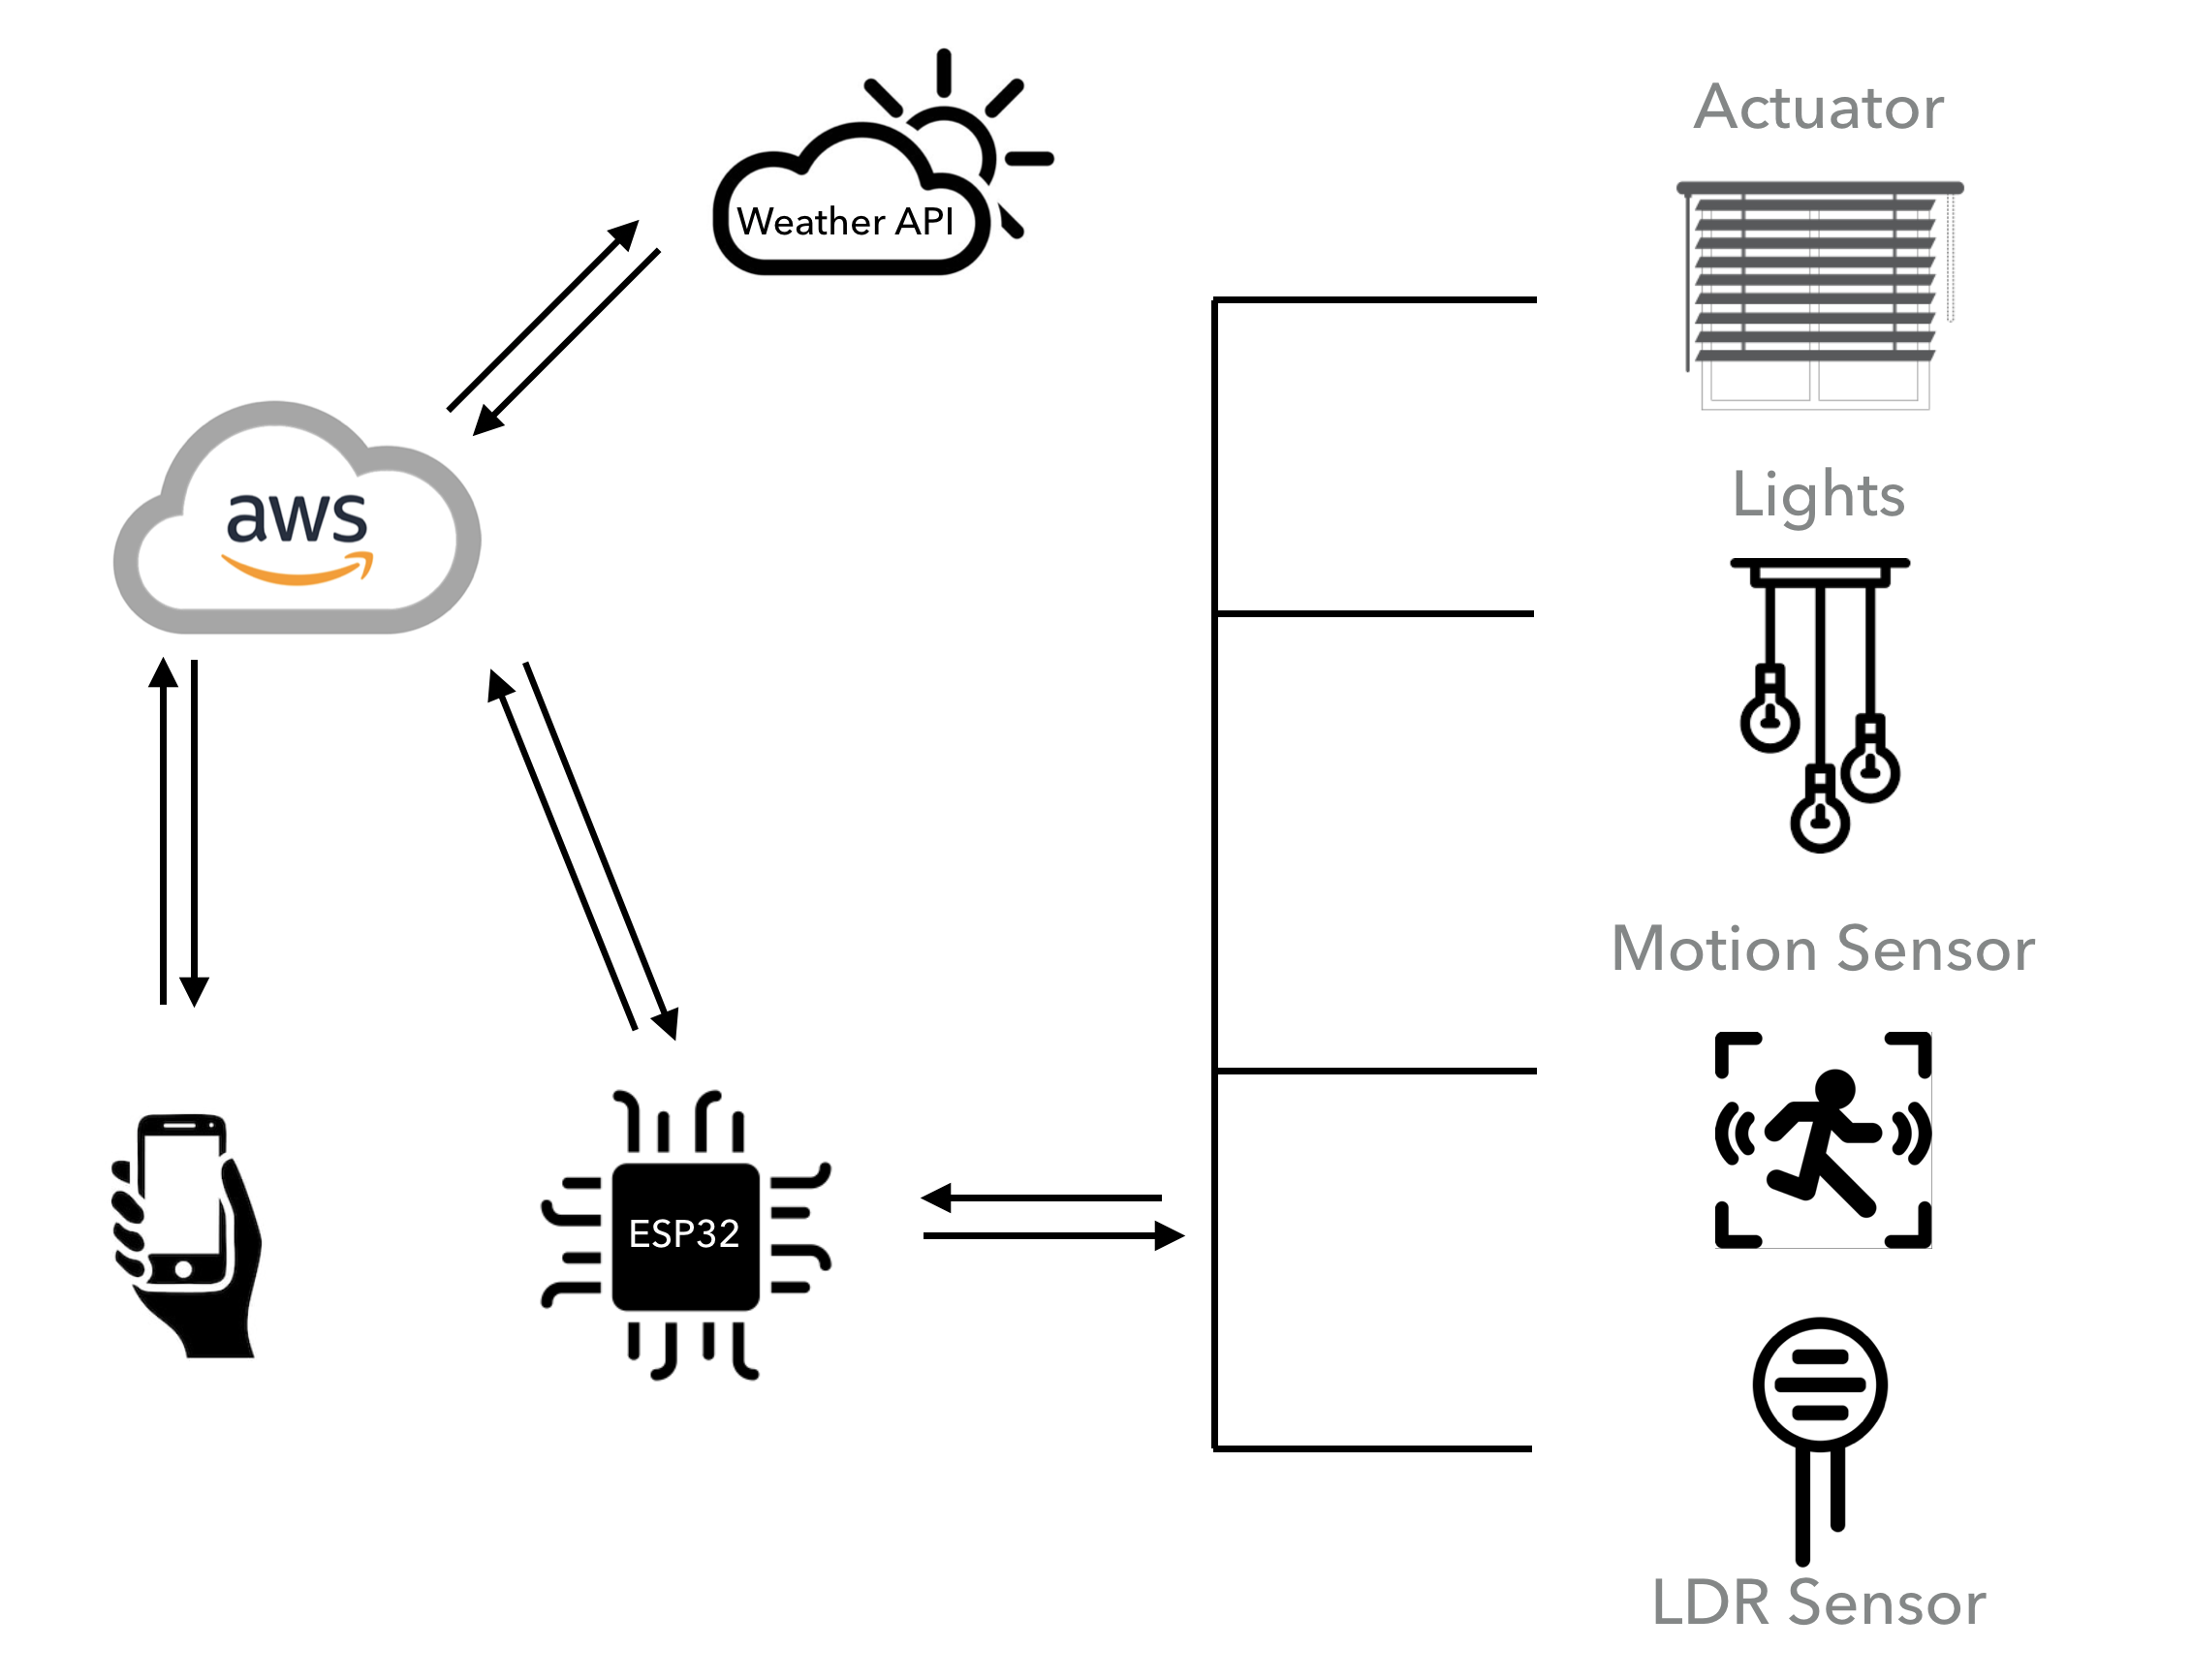
\includegraphics[scale=0.18]{Workflow.png}
	\caption{System workflow diagram}
\end{figure}

\section{Challenges and Future Enhancements}

Our major challenge during this project was the effects of COVID-19. Our team was not able to meet during the quarantine period. The professor could not give us the some of the hardware that was required to finish the project, and thus the gradual change in hue as it became darker could not be achieved as some of the diodes required another $5$V power supply. However, it was tried to achieve this gradual hue change with the use of only LEDs and that caused the ESP32 to hang at times. 
Power management is another major challenge that we faced during the development phase. The ESP32 is not powerful enough to power all the peripherals that were connected to it, hence there was some difficulty in managing the torque of the servo motor. The motor often struggled to lower/raise the blinds and sometimes when the motor was working, the intensity of the lights would drop indicating a lack of power. This requires an external power supply which we could not obtain during the development period due to COVID-19. The motor also did not allow rotation of 360{\textdegree}, instead, we were limited to movements between 0{\textdegree} to 180{\textdegree}.

The exact state of the bulb (on or off) is not saved on the cloud, and the same goes for the blinds as well. While using the AWS cloud to perform actions, the light and blinds are created as shadows \cite{aws_shadows}. When the MQTT broker needs to know the state of the object, it will query the shadow of the object and not the actual object itself [shadows]. Thus, if the internet connection is interrupted, then the shadow will return to its default state which is “OFF” for lights and “CLOSED” for blinds. Now the actual state of the object is lost, and this might cause communication errors. There was not enough time to fix this issue in this project.

The future scope of this project could include edge computing to reduce latency and make sure data stays close to the end nodes. It could also use some kind of an extender that allows for scalability of the number of peripherals that can be connected to the MCU. An external power supply would also make sure that enough power is being distributed to the peripherals.

\section{Conclusion}

This project shows that when technology is used right, it can benefit human beings greatly. An entirely automated smart lighting system for a house has been implemented with an added benefit of intrusion detection to ensure the safety of the house. The gradual dimming and hue change will help users relax and wind down for the day, thereby allowing them to sleep peacefully. Automated blinds make sure that the users do not have to be bothered with lowering the blinds before they sleep. In conclusion, this project demonstrates the various use cases of a real-life smart lighting system and with some modifications can be deployed in a real household.

\begin{thebibliography}{9}

\bibitem{esp32_doc} ESP32 Wroom 32 Datasheet, Version 2.9, \#101, Block 2, 690 Bibo Road, Zhangjiang High-Tech Park, Pudong, Shanghai, China 201203, 2020. 

\bibitem{ICCCE} S. N. Ibrahim, M. S. L. Hakim, A. L. Asnawi and N. A. Malik, "Automated Water Tank Filtration System Using LDR Sensor," 2016 International Conference on Computer and Communication Engineering (ICCCE), Kuala Lumpur, 2016, pp. 195-199. 

\bibitem{circadian} Sleepfoundation.org. 2020. What Is Circadian Rhythm? - National Sleep Foundation. [online] Available at: https://www.sleepfoundation.org/articles/what-circadian-rhythm [Accessed 1 April 2020].

\bibitem{blue_light} Chellappa, S.L., Steiner, R., Oelhafen, P., Lang, D., Götz, T., Krebs, J. and Cajochen, C. (2013), Acute exposure to evening blue‐enriched light impacts on human sleep. J Sleep Res, 22: 573-580. doi:10.1111/jsr.12050

\bibitem{sleep_org} sleep.org. What is the Sleep/Wake Cycle? [online] Available at: https://www.sleep.org/articles/sleepwake-cycle/  [Accessed 1 April 2020].

\bibitem{light} Czeisler, C. Perspective: Casting light on sleep deficiency. Nature 497, S13 (2013). https://doi.org/10.1038/497S13a

\bibitem{aws_iot} Amazon Web Services. AWS IoT Core [online] Available at: https://aws.amazon.com/iot-core/ [Accessed 1 April 2020].

\bibitem{esp_mqtt}  Amazon Web Services. AWS IoT Developer Guide - MQTT [online] Available at: https://docs.aws.amazon.com/iot/latest/developerguide/mqtt.html [Accessed 1 April 2020].

\bibitem{esp_aws} Explore Embedded. GitHub-Arduino-esp32-aws-iot [online] Available at: https://github.com/ExploreEmbedded/Hornbill-Examples/tree/master/arduino-esp32/AWS\_IOT [Accessed 1 April 2020].

\bibitem{aws_shadows} Amazon Web Services. AWS IoT Developer Guide - Using Shadows [online] Available at: https://docs.aws.amazon.com/iot/latest/developerguide/using-device-shadows.html [Accessed 1 April 2020].

\bibitem{esp_sec} Arduino. Securely Connecting an Arduino MKR WiFi 1010 to AWS IoT Core [online] Available at: https://create.arduino.cc/projecthub/Arduino\_Genuino/securely-connecting-an-arduino-mkr-wifi-1010-to-aws-iot-core-a9f365  [Accessed 1 April 2020].

\bibitem{android_pubsub} AWS Labs. GitHub-aws-sdk-android-samples [online] Available at: https://github.com/awslabs/aws-sdk-android-samples/tree/master/AndroidPubSub [Accessed 1 April 2020].

\end{thebibliography}
\vspace{12pt}
\end{document}
